\documentclass[paper=a4, fontsize=11pt]{scrartcl} % A4 paper and 11pt font size

%----------------------------------------------------------------------------------------
%	PACKAGES
%----------------------------------------------------------------------------------------
\usepackage[T1]{fontenc} % Use 8-bit encoding that has 256 glyphs
\usepackage{fourier} % Use the Adobe Utopia font for the document - comment this line to return to the LaTeX default
\usepackage[english]{babel} % English language/hyphenation
\usepackage{amsmath,amsfonts,amsthm} % Math packages
\usepackage{sectsty} % Allows customizing section commands
\usepackage{fancyhdr} % Custom headers and footers
\usepackage{tabularx, outlines, framed, varwidth, enumitem, graphicx, listings, color, qtree, float, subcaption, newfloat}
\usepackage[left=0.5in, right=0.5in, top=3in, bottom=.25in]{geometry}
\geometry{}

%----------------------------------------------------------------------------------------
%	SET CUSTOMIZATIONS AND FUNCTIONS
%----------------------------------------------------------------------------------------
\sectionfont{\centering \normalfont\scshape} % Make all sections centered, the default font and small caps
\pagestyle{fancyplain} % Makes all pages in the document conform to the custom headers and footers
\fancyhead{} % No page header - if you want one, create it in the same way as the footers below
\fancyfoot[L]{} % Empty left footer
\fancyfoot[C]{} % Empty center footer
\fancyfoot[R]{\thepage} % Page numbering for right footer
\renewcommand{\headrulewidth}{0pt} % Remove header underlines
\renewcommand{\footrulewidth}{0pt} % Remove footer underlines
\setlength{\headheight}{0pt} % Customize the height of the header

\DeclareFloatingEnvironment[fileext=lod]{diagram}

\numberwithin{equation}{section} % Number equations within sections (i.e. 1.1, 1.2, 2.1, 2.2 instead of 1, 2, 3, 4)
\numberwithin{figure}{section} % Number figures within sections (i.e. 1.1, 1.2, 2.1, 2.2 instead of 1, 2, 3, 4)
\numberwithin{table}{section} % Number tables within sections (i.e. 1.1, 1.2, 2.1, 2.2 instead of 1, 2, 3, 4)

\graphicspath{{./figures/}}
%\setlength\parindent{0pt} % Removes all indentation from paragraphs - comment this line for an assignment with lots of text

\makeatletter
	\newcommand*\variableheghtrulefill[1][.4\p@]
	{%
		\leavevmode
		\leaders \hrule \@height #1\relax \hfill
		\null
	}
\makeatother

\definecolor{codegreen}{rgb}{0,0.6,0}
\definecolor{codegray}{rgb}{0.5,0.5,0.5}
\definecolor{codepurple}{rgb}{0.58,0,0.82}
\definecolor{backcolour}{rgb}{0.97,0.97,0.97}
 
\lstdefinestyle{mystyle}{
    backgroundcolor=\color{backcolour},   
    basicstyle=\footnotesize,
    breakatwhitespace=false,         
    breaklines=true,                 
    captionpos=b,                    
    keepspaces=true,                 
%    numbers=left,                    
%    numbersep=5pt,                  
    showspaces=false,                
    showstringspaces=false,
    showtabs=false,                  
    tabsize=4
}

\lstdefinestyle{smallstyle}{
    %backgroundcolor=\color{backcolour},   
    basicstyle=\scriptsize,
    breakatwhitespace=false,         
    breaklines=true,                 
    captionpos=b,                    
    keepspaces=true,                 
%    numbers=left,                    
%    numbersep=5pt,                  
    showspaces=false,                
    showstringspaces=false,
    showtabs=false,                  
    tabsize=2
}
 
\lstset{style=mystyle}

%----------------------------------------------------------------------------------------
%	USEFUL COMMANDS
%----------------------------------------------------------------------------------------
%	\makebox[\textwidth][c]{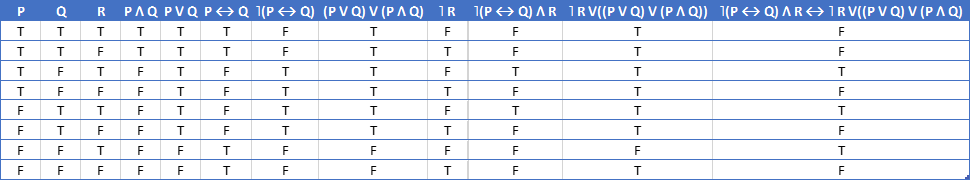
\includegraphics[width=.9\pagewidth]{p2-table}}

%	\newgeometry{top=.75in, bottom=.75in, left=.25in,right=.25in}
%	\newgeometry{top=.75in, bottom=.75in, left=1.25in,right=1.25in}

%	\lstinputlisting[firstline=4]{CMPSC360_Homework.cpp}

%\Tree
%	[.<root> [.<left> ][.<middle> ][.<right> ]]

%----------------------------------------------------------------------------------------
%	TITLE SECTION
%----------------------------------------------------------------------------------------

\newcommand{\horrule}[1]{\rule{\linewidth}{#1}} % Create horizontal rule command with 1 argument of height
% \title{Template: Homework 1}
\title{	
\normalfont \normalsize 
%\textsc{Rutgers University, Real Analysis I} \\ [25pt] % Your university, school and/or department name(s)
\horrule{0.5pt} \\[0.4cm] % Thin top horizontal rule
\huge STAT 461: Homework 2 \\ % The assignment title
\horrule{2pt} \\[0.5cm] % Thick bottom horizontal rule
}

\author{\textbf{\underline{Name:}}Kyle Salitrik | \textit{\textbf{\underline{ID\#:}} 997543474} | \textit{\textbf{\underline{PSU ID:}} kps168}} % Your name

\date{\normalsize\today} % Today's date or a custom date

\begin{document}

\maketitle % Print the title

%----------------------------------------------------------------------------------------
%	PROBLEM 1
%----------------------------------------------------------------------------------------
\newgeometry{top=.75in, bottom=.75in, left=1.25in,right=1.25in}
\section*{\variableheghtrulefill[.25ex]\quad Problem 1 \quad\variableheghtrulefill[.25ex]}
The following is the assignments for the first experiment:

\lstinputlisting[firstline=4]{listings/q1.txt}

%----------------------------------------------------------------------------------------
%	PROBLEM 2
%----------------------------------------------------------------------------------------

\section*{\variableheghtrulefill[.25ex]\quad Problem 2 \quad\variableheghtrulefill[.25ex]}
The following is the assignments for the second experiment:

\lstinputlisting[firstline=4]{listings/q2.txt}
%----------------------------------------------------------------------------------------
%	PROBLEM 3
%----------------------------------------------------------------------------------------

\section*{\variableheghtrulefill[.25ex]\quad Problem 3 \quad\variableheghtrulefill[.25ex]}
The following is the assignments for the third experiment:

\lstinputlisting[firstline=4]{listings/q3.txt}

%----------------------------------------------------------------------------------------
%	PROBLEM 4
%----------------------------------------------------------------------------------------

\section*{\variableheghtrulefill[.25ex]\quad Problem 4 \quad\variableheghtrulefill[.25ex]}
The first correlation was the lighthearted correlation of: US spending on science, space and technology correlated with Suicides by hanging, strangulation and suffocation. One thing interesting about this correlation is that with modern advancements in technology, it is easier to think of possible latent reasons for this correlation rather than counter-examples. 

However, on face value, simply increasing the spending budgets for science, space and technology wouldn't induce more suicides. One important piece of information left out is whether or not this spending budget has been adjusted to account for inflation. Even if the dollar amount goes up, it doesn't necessarily mean that the percentage of relative value has increased from the last year.

In contrast, one factor that could increase suicide rates would be the amount of automation implemented by advances in technology, which drives people out of jobs. These
forms of suicide are also fairly cheap to accomplish and the loss of income could push people who are already struggling in life over their breaking point.

%----------------------------------------------------------------------------------------
%	PROBLEM 5
%----------------------------------------------------------------------------------------

\section*{\variableheghtrulefill[.25ex]\quad Problem 5 \quad\variableheghtrulefill[.25ex]}

\subsection*{a)}
\begin{flalign*}
&W \sim N(2-3+0, 6+2+1)& \\
&W \sim  N(-1, 9) &
\end{flalign*}

\subsection*{b)}
\begin{flalign*}
&Q = 2Y; Y \sim N(-3, 2) &\\
&Q \sim N(2 * -3, 4 * 2) &\\
&Q \sim N(-6, 8) &
\end{flalign*}

\subsection*{c)}
\begin{flalign*}
&P = -2X + 4;\quad 4 \sim N(4,0);\quad X \sim N(-2, 6)&\\
&P \sim (-2*2, 4*6) + (4, 0) &\\
&P \sim (-4+4, 24 + 0) &\\
&P \sim N(0,24) &
\end{flalign*}

\subsection*{d)}
\begin{flalign*}
&X \sim N(2,6) &\\
&M \sim aX + b: M \sim (0,1) &\\
&M \sim N(a*2+b, a^2 * 6) &\\
&a = \sqrt{\frac{1}{6}} &\\
&b = -2*a &\\
&M \sim N \left(\sqrt{\frac{1}{6}} * 2 - \sqrt{\frac{1}{6}} * 2, \left(\sqrt{\frac{1}{6}}\right)^2 * 6 \right) &\\
&M \sim N(0, 1) &
\end{flalign*}


%----------------------------------------------------------------------------------------
%	PROBLEM 6
%----------------------------------------------------------------------------------------

\section*{\variableheghtrulefill[.25ex]\quad Problem 6 \quad\variableheghtrulefill[.25ex]}

\subsection*{a)}
\makebox[\textwidth][c]{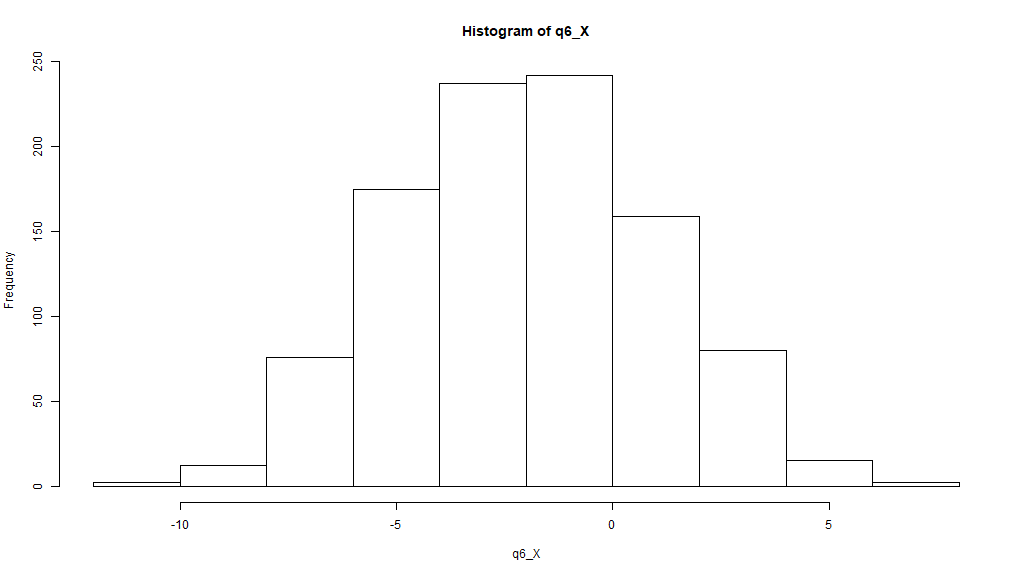
\includegraphics[scale=.5]{p6_a.png}}

\subsection*{b)}
\makebox[\textwidth][c]{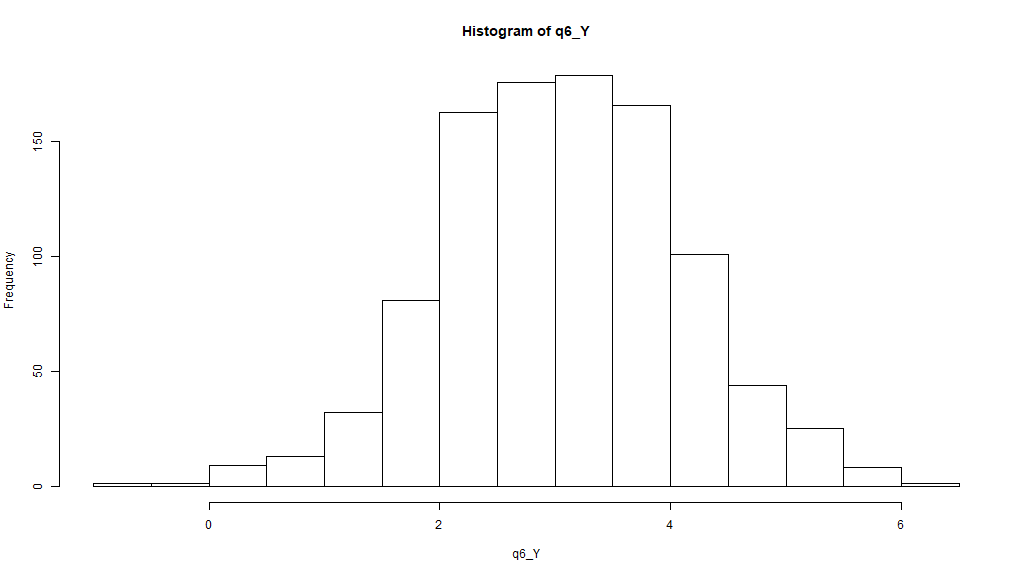
\includegraphics[scale=.5]{p6_b.png}}

\subsection*{c)}
\makebox[\textwidth][c]{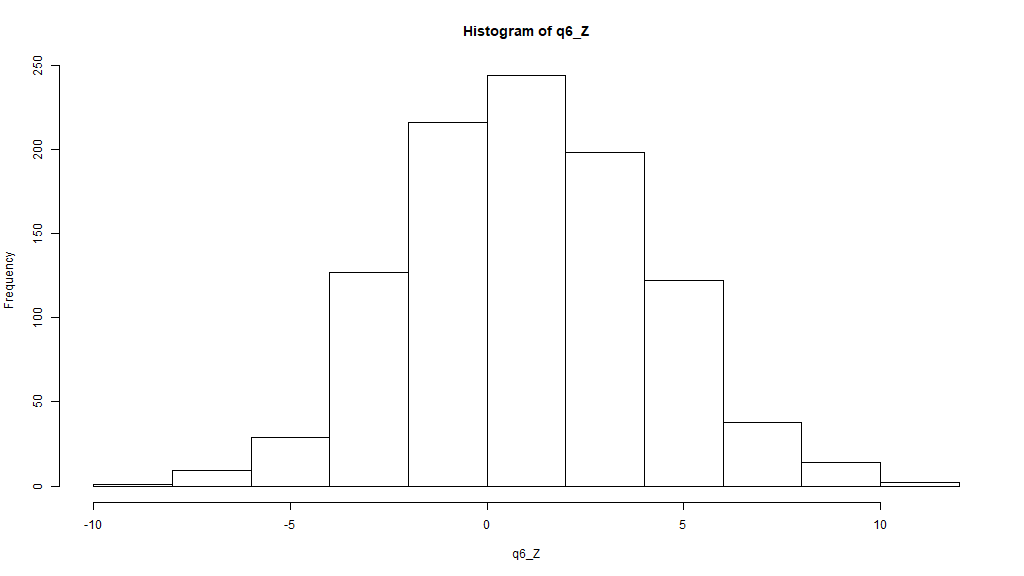
\includegraphics[scale=.5]{p6_c.png}}

\subsection*{d)}
Yes, although the distribution is a linear combination of the two independent distributions, the samples from Z are not dependent on samples from X or Y.
\begin{flalign*}
&P(Z|A,B) = P(Z) &\\
\end{flalign*}

\subsection*{e)}
\begin{flalign*}
&Z = X + Y; \quad X \sim N(-2, 3); \quad Y \sim N(3, 1) &\\
&Z \sim (-2 + 3, 3 + 1) &\\
&Z \sim (1, 4) &
\end{flalign*}	

\lstinputlisting[firstline=4]{listings/q6.txt}


\end{document}